\documentclass[tikz,border=5]{standalone}
\usetikzlibrary{positioning, matrix, arrows.meta,calc}

\begin{document}
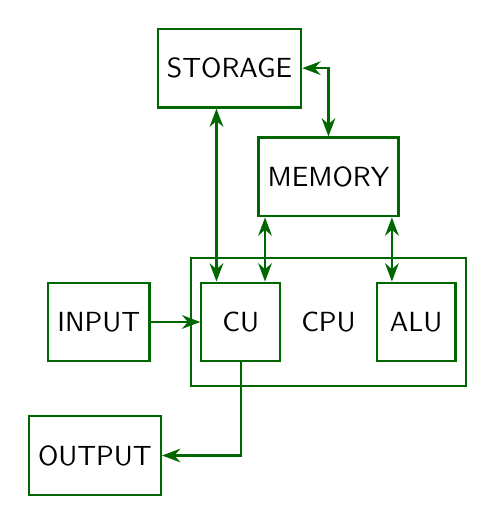
\begin{tikzpicture}[
    myline/.style={draw=green!40!black, thick},
    box/.style={myline, minimum height=1cm, minimum width=1cm, font=\sffamily, inner sep=.3333em}, >=Stealth]

    \matrix (CPU) [matrix of nodes, inner ysep=3mm, nodes=box, myline, column sep=1mm]
        {|(CU)|CU & |[draw=none]|CPU & |(ALU)| ALU \\};
    \node[box, left=5mm of CPU] (input) {INPUT};

    \node[box, below left=5mm of CPU] (output) {OUTPUT};
    \node[box, above=5mm of CPU] (memory) {MEMORY};
    \node[box, above left=5mm of memory, anchor=south] (storage) {STORAGE};

    \draw[<->, myline] (storage)-|(memory);
    \draw[->,myline] (input)--(CU);
    \draw[->,myline] (CU)|-(output);

    \draw[<->, myline] ($(CU.north west)!.2!(CU.north east)$) coordinate (aux)--(aux|-storage.south);
    \draw[<->, myline] ($(CU.north west)!.8!(CU.north east)$) coordinate (aux)--(aux|-memory.south);
    \draw[<->, myline] ($(ALU.north west)!.2!(ALU.north east)$) coordinate (aux)--(aux|-memory.south);
\end{tikzpicture}
\end{document}